\chapter{Zobecněné Paretovo rozdělení}\label{chap:gpd}
Přestože je normální rozdělení historicky často používané rozdělení v oblasti detekce novosti (zde bychom měli zmínit Grubbsův test \cite{grubbs} který se stal základním kamenem celé řady metod detekce novosti, resp. odlehlých vzorků), nemusí být vždy vhodné. Někdy může být střední hodnota a symetrický rozptyl zavádějící, ve smyslu výpovědní hodnoty o rozdělení sledovaných dat \cite{gpd4}. Zvláště, když je předmětem zájmu právě ocas rozdělení, z něhož data pocházejí. 
\par 
Uveďme zde Pickland - Balkema - de Haanovu větu \cite{gpd5,gpd6} (někdy označována jako druhá věta teorie extrémních hodnot) podle které, pro řadu $X_1$, $X_2$, $\dots$ nezávislých náhodných veličin se stejným rozdělením $F$ pro které je $F_u$ rozdělení jejich excesů přes mez $u$ (tedy hodnot které překračují $u$) platí
\begin{equation}
    F_u (x) \rightarrow GPD(\xi, \mu ,\sigma) (x), \text{ pro } u \rightarrow \infty
\end{equation}
kde $GPD$ je zobecněné Paretovo rozdělení a $F_u$ je distribuční funkce hodnot překračujících práh $u$ definovaná jako
\begin{equation}
    F_u(x)=P(X-u \leq x,X>u)=\frac{F(u+x)-F(u)}{1-F(u)}
\end{equation}
pro $0 \leq x \leq x_F-u$, kde $x_F$ je pravý koncový bod distribuční funkce $F$. Funkce hustoty pravděpodobnosti GPD je potom definovaná jako

\begin{equation}
  f_{(\xi,\mu,\sigma)}(x)=\begin{cases}
    \frac{1}{\sigma}\Bigg(1+\frac{\xi(x-\mu)}{\sigma}\Bigg)^{\Big(-\frac{1}{\xi}-1\Big)} & \text{for $\xi \neq 0$},\\
    \exp \Big(-\frac{x-\mu}{\sigma}\Big) & \text{for $\xi = 0$}.
  \end{cases}
\end{equation}
kde obecně $\mu \in (-\infty,+\infty )$ je parametrem lokace, $\sigma \in (0, \infty)$ je parametrem měřítka a $\xi \in (-\infty, \infty)$ je parametr tvaru. Odpovídající distribuční funkce je potom ve tvaru

\begin{equation}
  F_{(\xi,\mu,\sigma)}(x)=\begin{cases}
    1 - \Bigg(1+\frac{\xi(x-\mu)}{\sigma}\Bigg)^{-\frac{1}{\xi}} & \text{for $\xi \neq 0$},\\
    1 - \exp{\Big(-\frac{x-\mu}{\sigma} \Big)} & \text{for $\xi = 0$}.
  \end{cases}
\end{equation}
Důležitým faktem je, že nosič zobecněného Paretova rozdělení je omezený a to tak, že $x \geq \mu$ pro $\xi \geq 0$, a $\mu \leq x \leq \mu - \sigma/\xi$ pro $\xi < 0$ přičemž $\mu \in R$, $\sigma > 0$, a $\xi \in R$.
\par
Obrázek \ref{fig:gpd_pdfs} zobrazuje hustoty pravděpodobnosti GPD s různými parametry $\xi$, které mají demonstrovat možnosti použití GPD pro modelování různých typů ocasů. Pro $\xi=1$ je GPD ekvalentní s rovnoměrným rozdělením, pro hodnotu $\xi=0$ je exponenciálním rozdělením, pro $\xi=-0.5$ je trojúhelníkovým rozdělením, pro $-0.5 < \xi < 0$ je rozdělením s lehkým ocasem (např. normální rozdělení, Gumbelovo rozdělení), pro $\xi > 0$ je rozdělením s těžkým ocasem (např. Paretovo rozdělení, logaritmicko-normální rozdělení, Studentovo rozdělení) a pro $\xi < -1$ je rozdělením s kompaktním nosičem (např. beta rozdělení). Vzhledem k tomu, že v aplikacích s reálnými daty se vyskytuje celá řada rozdělení, je GPD, díky své výše demonstrované univerzalitě, vhodným rozdělením pro modelování ocasů jiných rozdělení \cite{gpd1,gpd2,gpd3}.

\begin{figure}
    \centering
    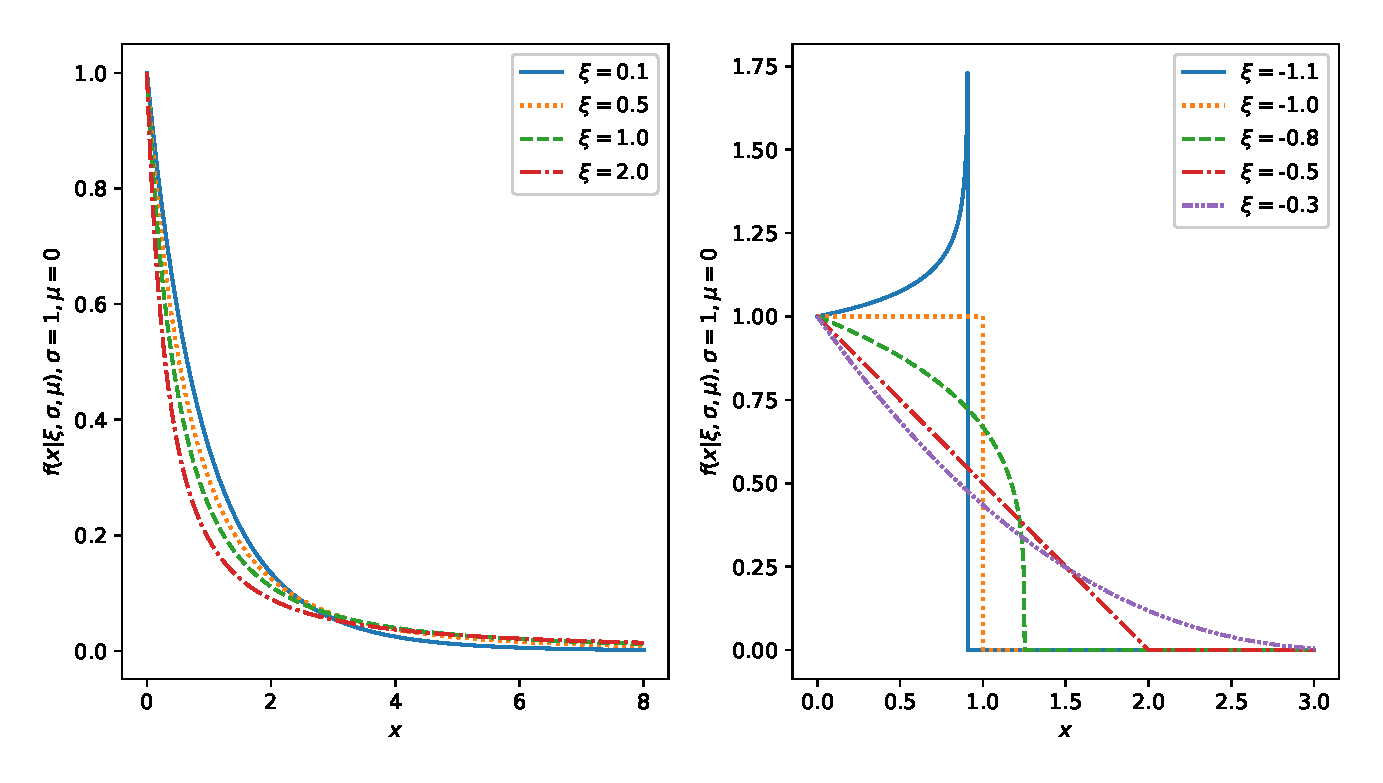
\includegraphics[scale=0.68]{IMG/MDPI/pdfs.eps}
    \caption{Hustoty pravděpodobnosti zobecněného Paretova rozdělení pro různé hodnoty parametru $\xi$ a zvolené hodnoty parametrů $\sigma=1$, $\mu=0$}
    \label{fig:gpd_pdfs}
\end{figure}

\section{Metoda Peak-over-Threshold}
Zásadním problémem při hledání parametrů GPD je volba vhodné hodnoty prahu $z$. Metody, které řeší uvedený problém, jsou nazývány Peak-Over-Threshold (POT). V případě, že je hodnota prahu $z$ příliš vysoká, jsou parametry GPD velmi proměnlivé, protože existuje příliš málo dat, které zvolenou prahovou hodnotu překročí. Pokud je hodnota prahu $z$ naopak příliš nízká, není aproximace ocasu generujícího rozdělení spolehlivá.  Z tohoto pohledu, je tedy vhodná volba hodnoty prahu $z$ pro kvalitu fitu GPD zásadní. Existuje celá řada metod pro výběr hodnoty prahu (více viz \cite{scarrott2012review}). Některé z metod POT jsou však výpočetně náročné, případně poskytují výsledky, jež musí být vyhodnoceny expertem. Z těchto důvodů nejsou příliš vhodné pro algoritmus detekce novosti, který by vyhodnocoval data v reálném čase. Proto se zdá vhodné využít některé z metod \textquote{Rule of Thumb}. Z těchto metod se osvědčily tři různé metody.
\par 
Nechť $l$ je počet vzorků, které jsou použity k odhadu parametrů GPD a $n_s$ je celkový počet vzorků, které jsou k dispozici. Potom podle \cite{DuMouchel,ferreira2003optimising,loretan1994testing} můžeme určit počet vzorků potřebných k odhadu parametrů GPD jako:
\begin{equation} \label{eq:l1}
    l_1=\ceil[\big]{0.1 \cdot n_s}
\end{equation}
\begin{equation} \label{eq:l2}
    l_2=\ceil[\big]{\sqrt{n_s}}
\end{equation}
\begin{equation} \label{eq:l3}
     l_3=\ceil[\bigg]{\frac{\sqrt[3]{n_s^{2}}}{log(log(n_s))}}
\end{equation}
Ještě poznamenejme, že pro odhad parametrů GPD se využívají vzorky s nejvyšší  hodnotou a symbolem $\ceil{\, }$ rozumíme horní celou část daného čísla.
\par
Metoda POT je zásadním prvkem v algoritmu Extreme Seeking Entropy (viz kapitola \ref{chap:ese}), kde je použita pro rozdělení přírůstku adaptivních vah filtru $|\Delta w_k(k)|$ do příslušných množin $H_i$ respektive $L_i$.


\section{Metody odhadu parametrů zobecněného Paretova rozdělení}
Odhad parametrů zobecněného Paretova rozdělení není triviální problém, proto existuje celá řada metod, které tento problém řeší. V následující textu je věnována pozornost metodě momentů (MOM) \cite{mom_orig}, metodě maximální věrohodnosti (ML) \cite{DuMouchel} a metodě kvazi-maximální věrohodnosti (QML) \cite{Luceno}. Z nověji publikovaných metod uveďmě alespon metodu věrohodných momentů \cite{zhang1}, metodu vážených nelineárních čterců momentů \cite{zhao,park}. Přehled dalších metod nabízí např. publikace \cite{gpd_est}.
\subsection{Metoda maximální věrohodnosti}
Metoda maximální věrohodnosti (maximum likelihood) je jednou ze zásadních statistických metod (pro zajímavost: byla použitá i Johannem Carlem Friedrichem Gaussem nebo Pierre-Simon Laplacem, více viz \cite{history}). Slouží k odhadu parametrů různých rozdělení pravděpodobnosti \cite{stat_bible}. Pro odhad parametrů je použita tzv. věrohodnostní funkce definovaná jako
\begin{equation}\label{eq:ml_arg}
\mathcal{L}(\theta|X_1,\dots,X_n)=\prod_{i=1}^n f(X_i|\theta)
\end{equation}
kde $\theta\in \Omega$ je vektor odhadu parametrů, $\Omega$ je množina parametrů rozdělení a $X_1$,...,$X_n$ je soubor nezávislých náhodných veličin se stejným rozdělením a neznámou hustotou pravděpodobnosti. Pro maximálně věrohodný odhad $\hat{\theta}$ pak platí
\begin{equation}
\hat{\theta}=arg \max_{\theta \in \Omega} \mathcal{L}(\theta|X_1,X_2,\dots,X_n).
\end{equation}
Tento vektor parametrů rozdělení tedy maximalizuje věrohodnostní funkci. V praxi se často pracuje s logaritmem věrohodnostní funkce, takže problém je formulován jako
\begin{equation}
\log \mathcal{L}(\theta|X_1,\dots,X_n)=\sum_{i=1}^n \log f(X_i|\theta)
\end{equation}

\par Věrohodnostní funkce pro zobecněné Paretovo rozdělení byla  zformulovaná DuMouchelem \cite{DuMouchel} ve tvaru
\begin{equation}\label{eq:ml}
\log\mathcal{L}(\sigma, \gamma|x_{1},\dots,x_{n})= -n \log \sigma +  \frac{1-\gamma}{\gamma}\sum_{i=1}^n\log\Big(1 - \frac{\gamma}{\sigma}(x_{i}-\mu)\Big)
\end{equation}
přičemž podle \cite{SmithML} je pro $-0.5 < \xi < 0$, při zachování určitých podmínek, maximálně věrohodný odhad asymptoticky normální a asymptoticky vydatný. Problém může pro hodnoty $\xi < -0.5$ kdy maximálně věrohodný odhad nemusí existovat \cite{grim}. Optimalizační problém \ref{eq:ml_arg}  pro GPD s věrohodností funkcí ve tvaru \ref{eq:ml} obvykle řeší nějakou numerickou metodou.
\subsection{Metoda momentů}
Při použití metody momentů (MOM)  je k odhadu parametrů GPD využito prvního a druhého momentu \cite{mom_orig}. 
Abychom poukázali na problém, který je s použitím MOM spojen, uvažujme nyní dvou parametrové GPD, pro které je $\mu=0$, $\xi > 0$ a $x \geq 0$. 
Pro první moment potom dostaneme přímo podle definice
\begin{equation*}
E(X)=\int_{0}^{\infty}x\frac{1}{\sigma}\Bigg(1+\frac{\xi x}{\sigma}\Bigg)^{\Big(-1-\frac{1}{\xi}\Big)}dx=\sigma^{\frac{1}{\xi}}\int_{0}^{\infty}x(\xi x + \sigma)^{-\frac{1}{\xi}-1}dx=\sigma^{\frac{1}{\xi}}\Bigg[-\frac{x}{(\xi x + \sigma)^{\frac{1}{\xi}}}\Bigg]_0^{\infty}-
\end{equation*}
\begin{equation*}
-\sigma^{\frac{1}{\xi}}\int_{0}^{\infty}-\frac{x}{(\xi x + \sigma)^{\frac{1}{\xi}}} dx=\sigma^{\frac{1}{\xi}}\Bigg[-\frac{x}{(\xi x + \sigma)^{\frac{1}{\xi}}}\Bigg]_0^{\infty} + \sigma^{\frac{1}{\xi}}\Bigg[\frac{(\xi x + \sigma)^{1-\frac{1}{\xi}}}{\xi(1-\frac{1}{\xi})}\Bigg]_0^{\infty}=
\end{equation*}
\begin{equation}
=\Bigg[\frac{\sigma^{\frac{1}{\xi}}(x+\sigma)}{(\xi-1)(\xi x+\sigma)^{\frac{1}{\xi}}}\Bigg]_0^{\infty}=\frac{\sigma}{1-\xi}
\end{equation}
přičemž z předposledního výrazu je patrné, že konečnou hodnotu získáme pouze pro hodnoty $0 < \xi < 1$. Obdobně pro rozptyl GPD 
\begin{equation*}
Var(X)=\int_{0}^{\infty}x^2 \frac{1}{\sigma}\Bigg(1+\frac{\xi x}{\sigma}\Bigg)^{\big(-1-\frac{1}{\xi}\big)}dx-\frac{\sigma^2}{(1-\xi)^2}=
\end{equation*}
\begin{equation}
=\Bigg[\frac{\sigma^{\frac{1}{\xi}}\big((\xi-1)x^2-2\sigma x-2\sigma^2\big)}{(\xi-1)(2\xi-1)(\xi x+\sigma)^{\frac{1}{\xi}}}  \Bigg]_0^{\infty}-\frac{\sigma^2}{(1-\xi)^2}=\frac{\sigma^2}{(1-\xi)^2(1-2\xi)}
\end{equation}
přičemž z předposledního výrazu je patrné, že konečnou hodnotu získáme pouze pro hodnoty $0 < \xi < 0.5$.
\par
Obecný $r$-tý moment GPD existuje pokud je splněna podmínka $\xi < 1/r$.
První čtyři momenty GPD (průměr, rozptyl, koeficienty šikmosti a špičatosti), jsou definovány jako
\begin{equation}\label{eq:mom1}
E(X)=\mu+\frac{\sigma}{1-\xi}
\end{equation}
\begin{equation}\label{eq:mom2}
Var(X)=\frac{\sigma^2}{(1-2\xi)(1-\xi)^2}
\end{equation}
\begin{equation}\label{eq:mom3}
Skew(X)=\frac{2(1+\xi)\sqrt{1-2\xi}}{1-3\xi}
\end{equation}
\begin{equation}
Kurt(X)=\frac{2(1-2\xi)(2\xi^2+\xi+3)}{(1-3\xi)(1-4\xi)}-3
\end{equation}
s přihlédnutím k omezení, že $\xi < 1/r$. Řešením soustavy rovnic \ref{eq:mom1} a \ref{eq:mom2} dostaneme odhady parametrů GPD jako
\begin{equation}
\sigma=\frac{1}{2}E(X)\Bigg(\frac{E(X)^2}{Var(X)}+1\Bigg)
\end{equation}
\begin{equation}
\xi=-\frac{1}{2}\Bigg(\frac{E(X)^2}{Var(X)-1}\Bigg)
\end{equation}
kde $E(X)$ je střední hodnota vzorku dat a $Var(X)$ je rozptyl tohoto vzorku dat. Metoda MOM je použitelná pouze pro hodnoty parametru $\xi < 0.5$. Pro $\xi \geq 0.5$ není splněná podmínka pro existenci druhého momentu. 

\subsection{Kvazi-ML metoda}
Kvazi-ML metoda  odhadu parametrů GPD kombinuje metodu maximální věrohodnosti pro $\xi > -0.75$ a modifikovanou metodu maximální věrohodnosti pro $\xi \leq -0.75$ \cite{Luceno}. Protože neznáme přesnou hodnotu parametru $\xi$ je rozhodnutí, kterou z metod použít provedeno na empirickém základě. Nejprve uvažujme posloupnost hodnot $(x_1,\dots, x_n)$. Metodu kvazi-ML lze popsat v následujících třech krocích.
\begin{enumerate}
\item Výpočet
\begin{equation}
\xi=\frac{-1}{n-1}\sum_{i=1}^{n-1} \ln \Big(1-\frac{x_1}{\max{x_1,\dots,x_n}}\Big)
\end{equation}
a
\begin{equation}
Z=1-\frac{\sum_{i=1}^n x_i}{2 n\overline{x}^2}
\end{equation}
kde $\overline{x}$ je střední hodnota posloupnosti hodnot $(x_1,\dots, x_n)$.
\item Pokud je $\xi<0.75$ a  $Z < 0.2$ použij metodu maximální věrohodnosti. 
\item Jinak určíme odhad parametru $\sigma$ jako
\begin{equation}
\sigma=\xi \cdot \max{(x_1,\dots,x_n)}
\end{equation}

\end{enumerate}
Z hlediska výpočetní náročnosti a možností hodnot, kterých může parametr $\xi$ nabývat, je uvedená hodnota dobrým kompromisem mezi metodou maximální věrohodnosti a metodou momentů.